%
% packets.tex
%
% Copyright The FloripaSat-2 Contributors.
%
% FloripaSat-2 Documentation
%
% This work is licensed under the Creative Commons Attribution-ShareAlike 4.0
% International License. To view a copy of this license,
% visit http://creativecommons.org/licenses/by-sa/4.0/.
%

%
% \brief EDC test report appendix.
%
% \author Gabriel Mariano Marcelino <gabriel.mm8@gmail.com>
%
% \version 0.9.0
%
% \date 2022/03/12
%

\chapter{EDC Test Report} \label{anx:edc-report}

This appendix is a test report of the EDC board.

\begin{itemize}
    \item \textbf{Date}: From 2022/03/03 to 2022/03/XX
    \item \textbf{Testers}: Bruno Benedetti, Gabriel M. Marcelino, Laio O. Seman
\end{itemize}

\begin{figure}[!htb]
    \begin{center}
        \subfigure[Top side.\label{fig:edc-top-test}]{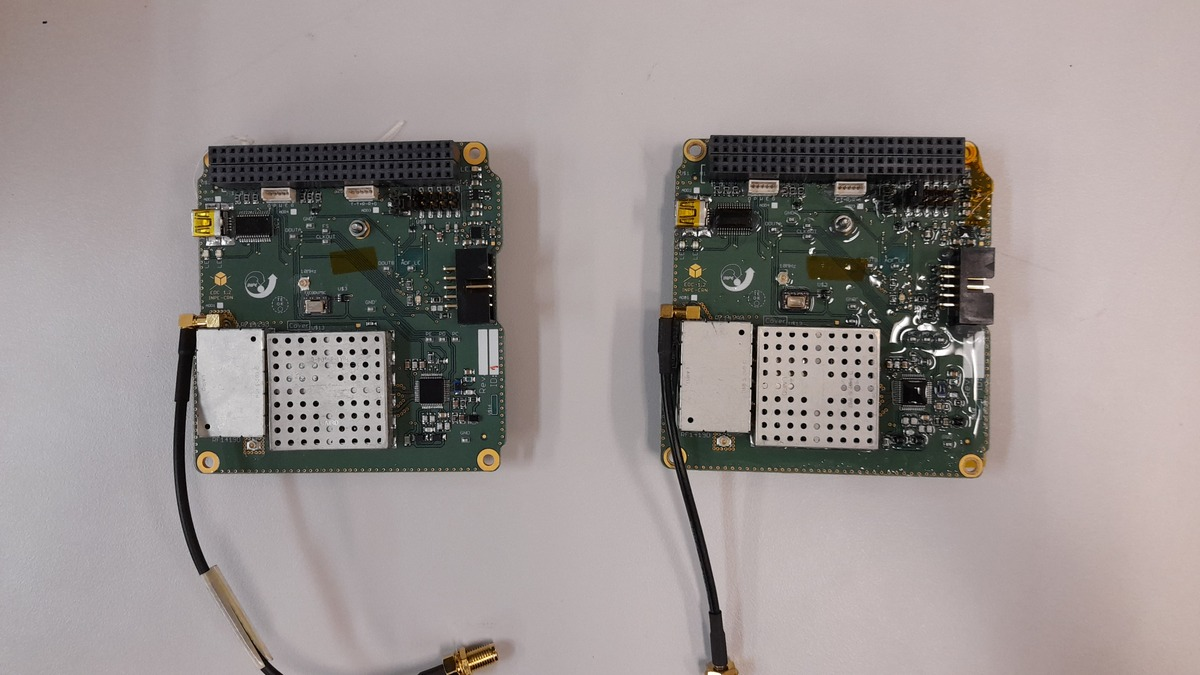
\includegraphics[width=\textwidth]{figures/edc_report/edcs-top}}

        \subfigure[Bottom side.\label{fig:edc-bottom-test}]{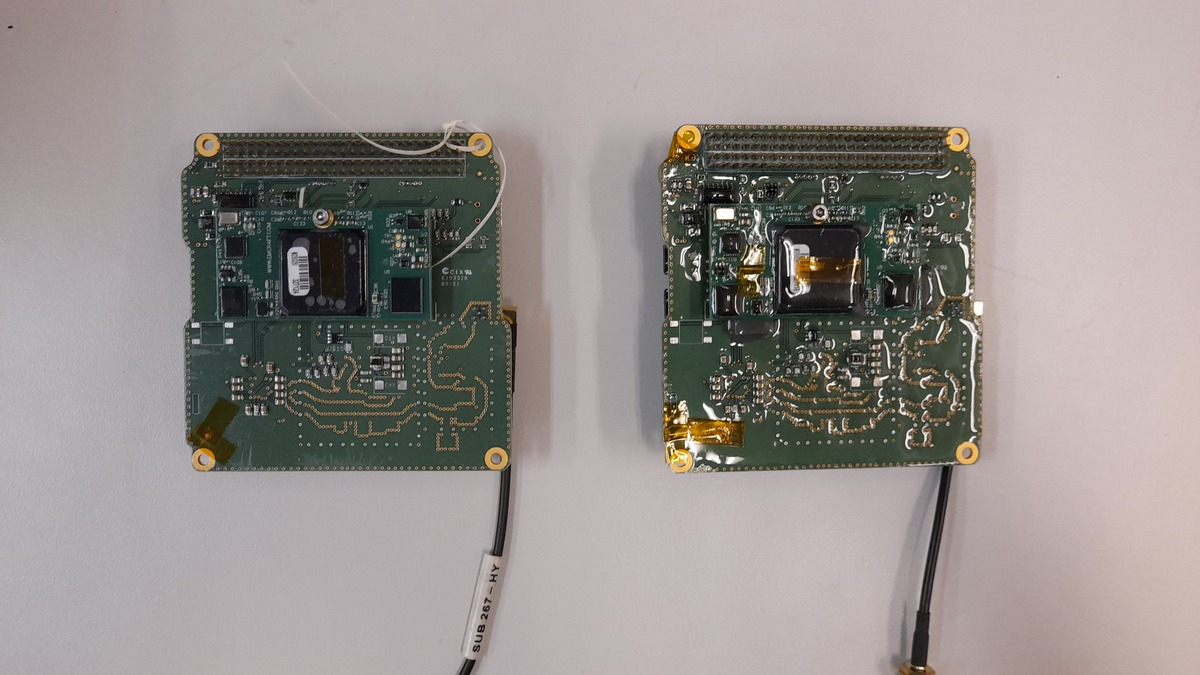
\includegraphics[width=\textwidth]{figures/edc_report/edcs-bottom}}
        \caption{Tested EDC boards.}
        \label{fig:edc-boards-test}
    \end{center}
\end{figure}

\section{Command interface test}

\subsection{Used material}

\begin{itemize}
    \item EDC boards
    \item USB-UART coverter
    \item Saleae Logic Analyzer
    \item Protoboard
    \item Desktop computer
    \item Logic 2 software
    \item Cutecom software
    \item USB cables
    \item Pin header wires
\end{itemize}

\begin{figure}[!ht]
    \begin{center}
        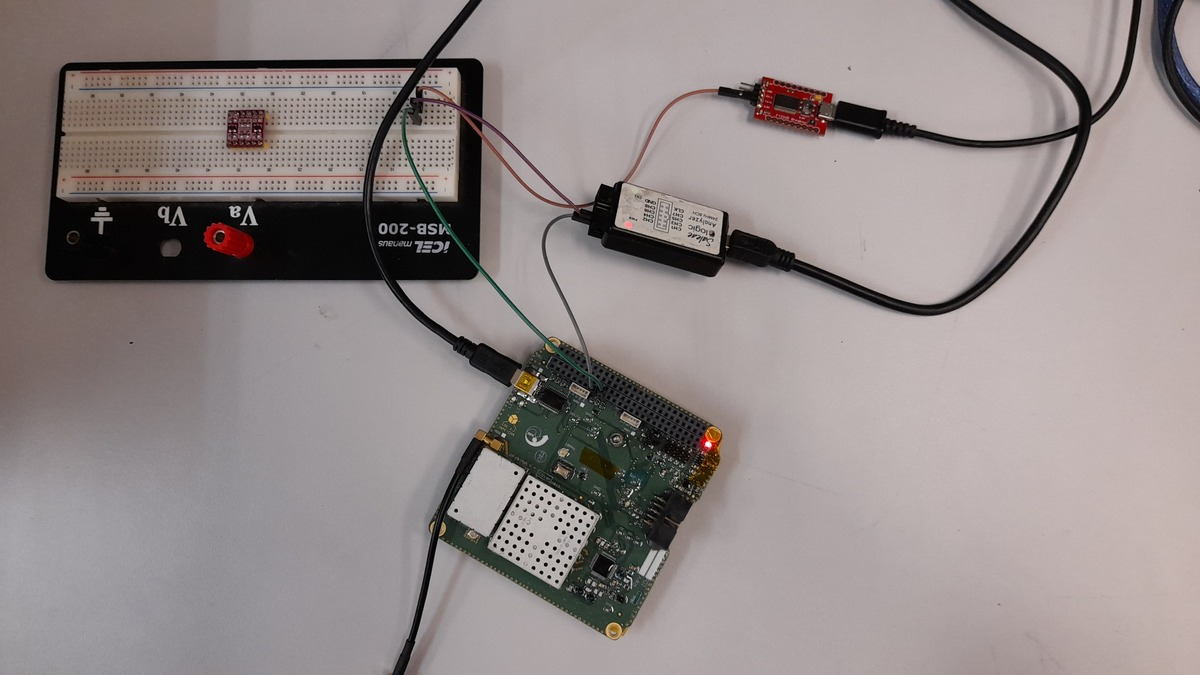
\includegraphics[width=\textwidth]{figures/edc_report/cmd-test-setup}
        \caption{Setup of the EDC's command interface test.}
        \label{fig:edc-test-setup}
    \end{center}
\end{figure}

\subsection{Results}

\begin{figure}[!ht]
    \begin{center}
        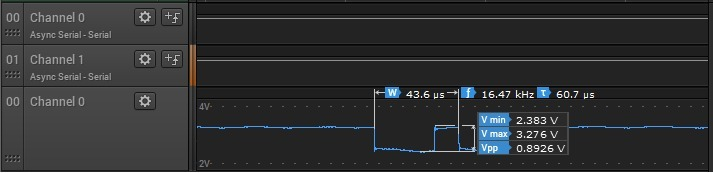
\includegraphics[width=\textwidth]{figures/edc_report/edc-cmd-issue}
        \caption{Command interface issue.}
        \label{fig:edc-cmd-issue}
    \end{center}
\end{figure}

\begin{figure}[!ht]
    \begin{center}
        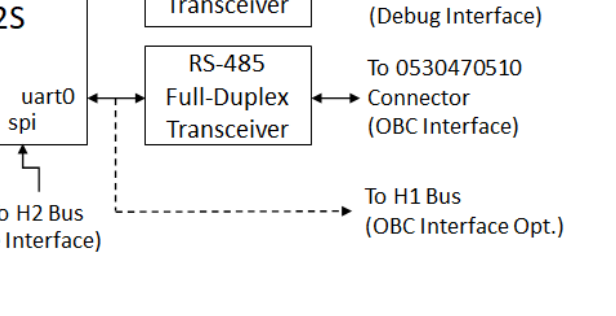
\includegraphics[width=0.6\textwidth]{figures/edc_report/edc-bd-uart-if}
        \caption{UART and RS-485 interfaces of the EDC.}
        \label{fig:edc-bd-uart-if}
    \end{center}
\end{figure}

\begin{figure}[!ht]
    \begin{center}
        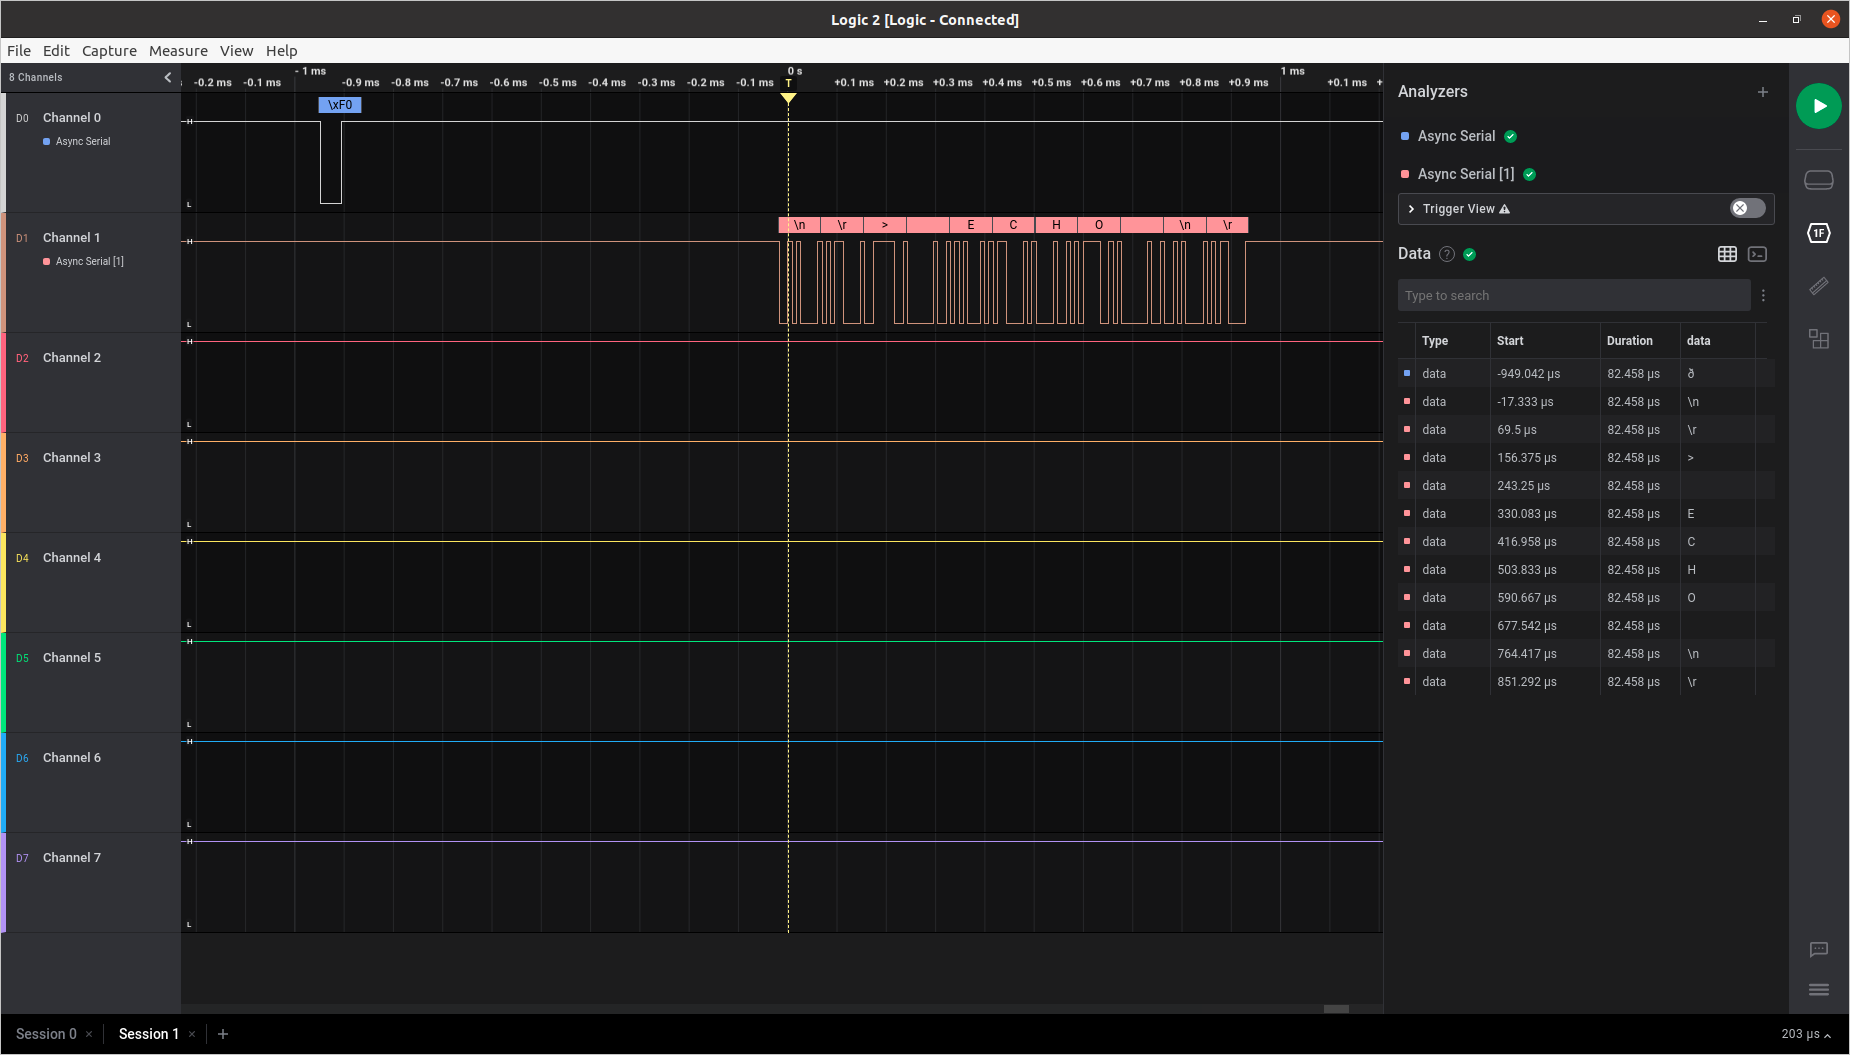
\includegraphics[width=\textwidth]{figures/edc_report/echo-cmd}
        \caption{``Echo'' command demonstration.}
        \label{fig:edc-echo-cmd}
    \end{center}
\end{figure}

\section{RF chain test}

\subsection{Used material}

\begin{itemize}
    \item EDC boards
    \item USB-UART converter
    \item Ettus USRP B210 SDR
    \item Desktop computer
    \item GNURadio v3.9
    \item Cutecom software
    \item USB cables
    \item Pin header wires
    \item SMA coaxial cable
    \item 30 dB attenuator
\end{itemize}

\begin{figure}[!ht]
    \begin{center}
        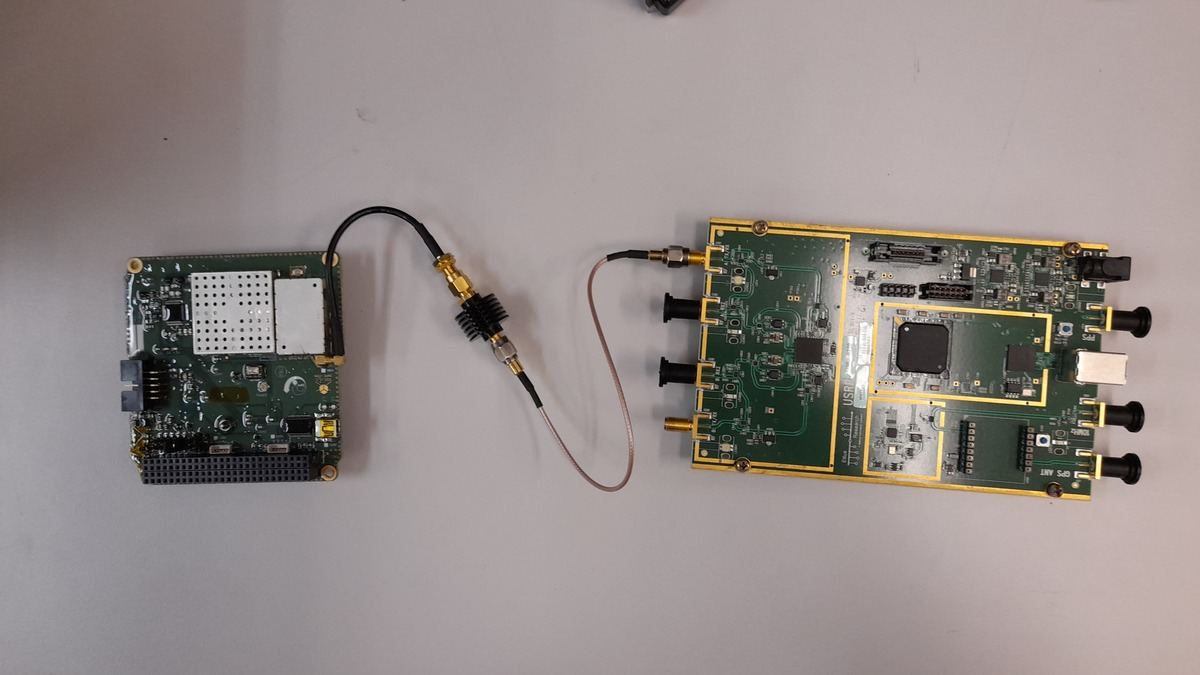
\includegraphics[width=\textwidth]{figures/edc_report/rf-chain-setup}
        \caption{Setup of the EDC's RF chain test.}
        \label{fig:edc-rf-chain-test-setup}
    \end{center}
\end{figure}

\begin{figure}[!ht]
    \begin{center}
        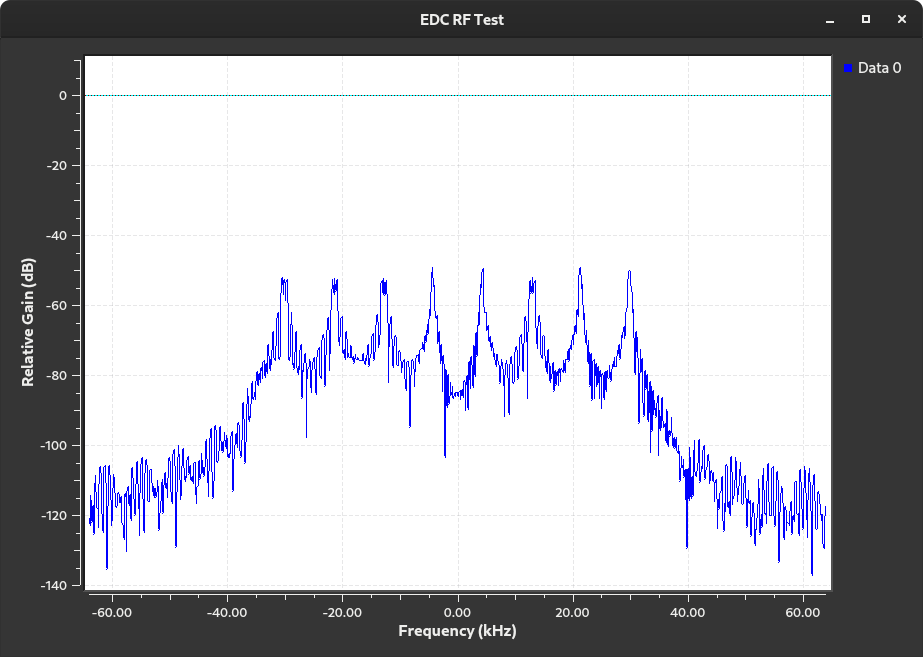
\includegraphics[width=\textwidth]{figures/edc_report/edc-rf-test-signal}
        \caption{Generated signal used in the RF chain test.}
        \label{fig:edc-rf-signal}
    \end{center}
\end{figure}

\subsection{Results}

.

\section{Conclusion}

.
